\documentclass[conference]{IEEEtran}
\usepackage{fontspec}
\setmainfont{Times New Roman}
\usepackage{amsmath}
\usepackage{amssymb}
\usepackage{graphicx}
\usepackage{booktabs}
\usepackage{microtype}
\usepackage{url}
\usepackage{balance}
\graphicspath{{figures/}}
\setlength{\textfloatsep}{7pt plus 1pt minus 2pt}
\setlength{\floatsep}{7pt plus 1pt minus 2pt}

\title{Reproducible Target-Informed Gaussian-Process Optimization for Data-Efficient Electromagnetic Design}
\author{\IEEEauthorblockN{Le Dong}
\IEEEauthorblockA{\textit{School of Electrical Engineering}\\
\textit{Xi'an Jiaotong University}\\
Xi'an, Shaanxi 710049, China\\
leroi\_2024@stu.xjtu.edu.cn}}

\begin{document}
\maketitle

\begin{abstract}
We study constrained electromagnetic design in which the final selected design must satisfy a prescribed response band while minimizing a second, possibly composite objective. Matched numerical experiments select Gaussian-process (GP) active learning and constrained expected improvement (cEI), then make initialization, GP fitting, call accounting, and stopping deterministic. The final workflow uses a center start, feasibility--uncertainty discovery, a $2d+1$ minimum-evidence guard, and a three-refit 1\% relative-cEI condition before a separately charged confirmation batch. Frozen after 14 development targets, it recovers all 73 remaining exhaustive optima on a 1,110-design coil lattice with 21.81 mean calls. On a frozen 21-target, eight-dimensional wireless-power-transfer (WPT) sweep, both the workflow and matched-budget conventional cEI qualify 21/21 targets, versus 10/21 for Sobol search. In a separate matched 1000-nH Maxwell execution, both policies use 30 accepted evaluations; the automatic workflow returns $0.38368~\Omega$ versus $0.38954~\Omega$. This single field-solver pair demonstrates executable transfer, not general dominance or wall-clock acceleration.
\end{abstract}

\begin{IEEEkeywords}
active learning, air-core coil, Gaussian process regression, surrogate optimization, simulated annealing, uncertainty quantification.
\end{IEEEkeywords}

\section{Introduction}
Electromagnetic design tasks often require repeated simulations or measurements while satisfying a compulsory performance target and optimizing another indicator. In general, let an expensive oracle return a constrained response $g(x)$ and a scalar objective $J(x)$. The design problem is
\begin{equation}
 \min_{x\in\mathcal X}J(x)\quad\mathrm{s.t.}\quad
 |g(x)-g_t|/|g_t|\leq\epsilon .
\end{equation}
$J$ may be a single quantity such as winding resistance or a scalarized function of loss, mass, temperature, material use, and efficiency. The acquisition logic is unchanged as long as the oracle supplies the chosen scalar objective. Here, the controlled benchmark targets inductance and minimizes resistance. Enumeration is possible only because the first domain is small; equal oracle-call budgets provide the experimental cost abstraction.

Although the principal benchmarks use DC winding resistance, the dual-response formulation is not restricted to analytically available quantities. In higher-fidelity WPT design, $J$ may represent frequency-dependent AC winding loss $P_{\rm AC}(x;f,\mathbf I)$ or an equivalent resistance obtained from an impedance matrix, incorporating skin and proximity effects under specified frequency and coil currents. Maxwell supports separate \texttt{SolidLoss} outputs for solid windings, while \texttt{StrandedLossAC} is specific to supported Litz-wire models \cite{ansysloss}. Then $g(x)\sim\mathcal{GP}_g$ and $J(x)\sim\mathcal{GP}_J$, while $a_{\rm cEI}=p_F\mathrm{EI}_J$ is unchanged. The numerical benchmarks deliberately hide both responses behind an oracle; a final direct Maxwell experiment tests whether the frozen workflow can operate with field-solved $M$ and AC self-resistance.

The experiments progress from reusable-surrogate and acquisition selection to deterministic target-specific budgeting and an 8-D mixed-integer continuous WPT transfer. The contributions are: (i) matched model and acquisition comparisons; (ii) an auditable workflow combining deterministic feasibility discovery and GP fitting with $B=N_0+N_{\rm seq}+N_{\rm conf}$ accounting and guarded stopping; and (iii) exhaustive held-out 2-D validation, a 21-target numerical WPT transfer, and a matched-budget direct Maxwell demonstration. This is a reproducibility and budget-control contribution, not a claim to have invented cEI or GP active learning.

\section{Related Work and Positioning}
Online surrogate-assisted electromagnetic optimization is well established. SADEA couples an online GP to differential evolution for antenna design \cite{liu2014}, and recent antenna workflows combine learned representations with GPs \cite{wu2024}. BO has also optimized ferrite-assisted WPT coils and frequency for efficiency \cite{sim2023}, while the 14-input model used here predicts mutual inductance over geometry and pose \cite{asadi2025}. Unlike these studies, we jointly audit target-specific feasibility discovery, deterministic fitting, posterior stopping, and a separately charged terminal evidence batch.

Initial-design size and placement affect low-budget BO \cite{furuuchi2024}, while formal stopping work values another observation through posterior simple-regret reduction \cite{ishibashi2023}. Our simpler three-refit relative-cEI threshold is an engineering heuristic validated exhaustively on the 2-D lattice, not the theoretically optimal rule of \cite{ishibashi2023}. The distinction is the frozen workflow and explicit budget accounting, not a new acquisition or stopping theory.

\section{Coil Model and Problem Formulation}
The coil geometry is described by radial layers $T$ and turns per layer $n$, with $N=Tn$. With wire diameter $d=0.68$~mm, pitch $p=1.05d$, inner diameter $D_0=80$~mm, $D=D_0+Tp$, height $H=np$, and radial thickness $C=Tp$, the deterministic oracle is $L=0.08N^2D^2,10^{-4}/(3D+9H+10C)$ mH and $R=4\rho ND/d^2$, where $\rho=1.851\times10^{-5}~\Omega\cdot\mathrm{mm}$. It therefore maps $(T,n)$ to $(L,R)$ without fitted parameters.

The evaluated rectangular domain uses $1\leq T\leq10$ and $20\leq n\leq130$, yielding $10\times111=1{,}110$ integer configurations. Total turn count is the derived quantity $N=Tn\in[20,1300]$; no independent upper bound on $N$ is imposed in this benchmark. For target $L_t$, a configuration is feasible if
\begin{equation}
 \frac{|L-L_t|}{L_t}\leq\epsilon,\qquad
 \epsilon=\frac{0.5\ \mathrm{mH}}{20\ \mathrm{mH}}=0.025.
\end{equation}
The objective is minimum resistance among feasible configurations. Exhaustive enumeration independently supplies the reference $R_{\mathrm{exhaustive}}$. For a feasible returned design, relative regret and the reported bounded loss are
\begin{equation}
 r=\frac{R}{R_{\mathrm{exhaustive}}}-1,\qquad u=\frac{r}{1+r}.
\end{equation}
Lower $u$ is better; an infeasible design is assigned $u=1$.

\section{Methods}
\subsection{Reusable Gaussian-Process Surrogate}
Independent GPs model both responses, $L(x)\sim\mathcal{GP}_L$ and $R(x)\sim\mathcal{GP}_R$, using anisotropic radial-basis-function kernels with white-noise terms \cite{rasmussen}. Predictive means supply $\mu_L$ and $\mu_R$, while posterior standard deviations quantify epistemic uncertainty. The random-sampling variant trains on 17 seeded uniform samples. The uncertainty-sampling variant starts from six samples and selects 11 additional configurations using the target-independent criterion
\begin{equation}
a_{\mathrm{G}}(x)=(1-\alpha)\frac{\sigma_L(x)}{s_L}
 +\alpha\frac{\sigma_R(x)}{s_R},\quad 0\leq\alpha\leq1,
\end{equation}
where the positive scales $s_L$ and $s_R$ are fixed after the initial design. The matched comparison uses $\alpha=0.5$. Because $a_{\mathrm{G}}$ contains no requested target, feasible incumbent, or objective improvement, the learned model remains reusable for all $L_t$. After either policy, ten final evaluations maximize $s_{\rm ver}(x)=p_F(x)\exp[-\operatorname{unit}(\mu_R(x))]$, where $\operatorname{unit}$ denotes candidate-wise min--max scaling.

\subsection{Ten-Network Ensemble}
The neural alternative fits separate ten-member ensembles for $L$ and $R$. Each member is an independently initialized, L2-regularized MLP with hidden layers of 16 and 8 ReLU units. Ensemble means supply the response predictions and member disagreement supplies empirical uncertainty \cite{lakshminarayanan}. Its random and uncertainty-sampling variants use exactly the same sample counts, balanced criterion, validation score, and decision pool as the GP variants. This matched construction separates the effects of model family and active selection.

\subsection{Direct Stochastic Search}
Simulated annealing (SA), genetic algorithm (GA), and particle swarm optimization (PSO) search the integer grid directly. Repeated configurations are cached. A common stopping criterion requires a feasible solution and then stops after five cycles without a $\geq1\%$ reduction in the best feasible resistance; a full-domain safety cap remains available. The algorithms respectively use probabilistic local moves, population evolution, and particle updates \cite{kirkpatrick,holland,kennedy}.

\subsection{Target-Conditioned GP Optimization}
This third class also evaluates the physical model sequentially, but differs from direct search because two GPs are fitted and their acquisition function selects each subsequent evaluation. For target $L_t$, the inductance GP supplies the two-sided feasibility probability
\begin{equation}
\begin{aligned}
p_F(x)&=\Phi\!\left(\frac{L_t(1+\epsilon)-\mu_L(x)}{\sigma_L(x)}\right)\\
&\quad-\Phi\!\left(\frac{L_t(1-\epsilon)-\mu_L(x)}{\sigma_L(x)}\right).
\end{aligned}
\end{equation}
Three established local acquisitions are compared. Constrained expected improvement uses $a_{\mathrm{cEI}}=p_F\mathrm{EI}_R$, with $p_F$ alone before a feasible incumbent exists \cite{gardner}. Constrained lower confidence bound uses
\begin{equation}
\begin{aligned}
\ell_R(x)&=\mu_R(x)-\kappa\sigma_R(x),\\
a_{\mathrm{cLCB}}(x)&=p_F(x)\exp[-\operatorname{unit}(\ell_R(x))].
\end{aligned}
\end{equation}
where $\operatorname{unit}$ is min--max normalization over unseen candidates and $\kappa=2$. Thus $-\ell_R=-\mu_R+\kappa\sigma_R$: uncertainty increases the maximized score, as required by conventional LCB exploration \cite{srinivas}. Weighted integrated variance reduction (IVR) selects the point expected to reduce posterior variance across a quadrature set mixing the whole domain with the current target-relevant region, following the integrated-variance principle of active design \cite{cohn}.

This comparison deliberately uses pure target-conditioned acquisitions. It therefore tests whether the requested constraint should guide sampling, rather than simultaneously introducing a global--local mixture. The acquisition is rerun independently for every $L_t$, trading a reusable global model for target-specific precision.

\subsection{Deterministic Feasibility Start}
Ordinary cEI requires a feasible incumbent. Its conventional fallback maximizes $p_F$, but a GP fitted to one central observation can become locally confident before learning which direction reaches a distant target. We therefore evaluate the normalized domain center first and, until feasibility is observed, use
\begin{equation}
 a_F(x)=\omega\,\operatorname{unit}(p_F(x))
 +(1-\omega)\,\operatorname{unit}(\sigma_L(x)).
 \label{eq:feasibility-start}
\end{equation}
The working default is $\omega=0.75$. Larger $\omega$ is more conservative, emphasizing predicted feasibility; smaller $\omega$ is more exploratory. Once a feasible point is observed, the rule switches to ordinary cEI without an auxiliary term. Kernel hyperparameters are held at declared prior values for the first three observations and optimized thereafter, avoiding poorly identified one-point length-scale fitting.

Random optimizer restarts are also unnecessary. From the fourth observation onward, kernel marginal likelihood is optimized from the declared prior and four fixed Halton points spanning the bounded log-hyperparameter domain. The best of these $K=5$ L-BFGS-B solutions is retained. Thus $K$ is a transparent surrogate-computation allowance, while identical physical observations yield identical GPs.

After feasibility, let $R_k^*$ be the best feasible resistance after refit $k$. We monitor the maximum candidate-wise relative cEI,
\begin{equation}
 \rho_k=\max_{x\in\mathcal C_k}
 \frac{p_F(x)\mathrm{EI}_R(x)}{R_k^*}.
 \label{eq:stopping}
\end{equation}
The active phase may stop only after at least $N_{\min}=2d+1$ model-building observations, where $d$ is the optimized input dimension, and when $\rho_k\leq\delta=0.01$ for three consecutive refits. The dimension-aware guard prevents a very small initial sample from terminating solely because its GP is overconfident; it is an engineering minimum, not a sample-complexity theorem. The cEI condition means that, under the fitted posterior and searched candidate set, the largest probability-weighted expected reduction is at most 1\% of the incumbent resistance. It is not a bound on the unknown global-optimality gap: an overconfident or misspecified GP can make $\rho_k$ small inside a local basin. The minimum-evidence guard, three-refit patience, candidate-wide maximization, retained posterior uncertainty, and the terminal evidence batch reduce that risk but cannot eliminate it. Stopping ends adaptive model building but retains ten same-oracle confirmations ranked by $p_F\exp[-\operatorname{unit}(\mu_R)]$; the final decision is the lowest observed feasible resistance over both phases.

\subsection{Eight-Dimensional Nominal WPT Design}
The source WPT model has 14 inputs: eight intrinsic coil variables and six relative-pose variables \cite{asadi2025}. For each transmitter and receiver, the geometric variables are polygon side count $n_s\in[4,10]$, turn count $n_t\in[5,15]$, inter-turn spacing $s\in[1,3]$~mm, and inner radius $r_i\in[30,80]$~mm. We optimize this eight-dimensional mixed-integer continuous geometry: $n_s$ and $n_t$ are integral, while $s$ and $r_i$ are continuous. Translation is fixed at $(0,0,70)$~mm and all three rotations at zero. Thus no misalignment or tolerance variable is optimized, and no robustness-to-deviation claim is made.

For requested mutual inductance $M_t$, the constraint is $|M(x)-M_t|/M_t\leq0.025$; the objective is total copper winding resistance. The 1500-nH case is retained for the representative geometry. Integer variables are rounded before evaluation and continuous variables retain their sampled values. For coil $q\in\{t,r\}$, turn $k$ has circumradius $r_{q,k}=r_{i,q}+k(s_q+w)$ and polygonal length $2n_{s,q}r_{q,k}\sin(\pi/n_{s,q})$. Thus
\begin{equation}
 R=\frac{\rho_{\rm Cu}}{A}\sum_{q\in\{t,r\}}\sum_{k=0}^{n_{t,q}-1}
 2n_{s,q}r_{q,k}\sin(\pi/n_{s,q}),
\end{equation}
with circular conductor diameter $w=0.68$~mm, $A=\pi(w/2)^2$, and $\rho_{\rm Cu}=1.851\times10^{-5}~\Omega\,{\rm mm}$. Radii and lengths in this equation are in millimetres; leads and interconnections are excluded. The partial-inductance oracle follows the source model.

Here $R=R_t+R_r$ is an unweighted geometry metric. It has a normalized copper-loss interpretation when the RMS coil currents are equal, since then $P_{\rm Cu}=I^2(R_t+R_r)$. Comparable Tx/Rx currents are plausible for a symmetric, resonantly tuned, approximately efficiency-matched series--series link: maximum-efficiency analysis relates their resonant-current ratio to the primary and secondary equivalent series resistances, so near-identical resistances give a ratio near unity \cite{zhang2019mept}. Equality is nevertheless not imposed as a general operating fact; load, compensation, and off-design operation can change the ratio. The benchmark therefore uses $R_t+R_r$ as a circuit-independent coil-material proxy, whereas deployment may replace it with current-weighted or field-solved loss without changing the acquisition logic.

For the automated transfer, the first design is the geometric center $(7,10,2,55,7,10,2,55)$. Candidate blocks are consecutive segments of one unscrambled Sobol sequence, so no pseudorandom candidate seed remains. The two response GPs use isotropic Mat\'ern-$5/2$ kernels: prior hyperparameters are fixed for fewer than four observations and thereafter use the same deterministic $K=5$ optimizer. The 75/25 feasibility rule, ordinary cEI, $\delta=1\%$, three-refit patience, and ten-confirmation rule are transferred unchanged from the 2-D development problem.

\section{Experimental Protocol}
Targets are the integers 1--87 mH. Every stochastic method uses seeds 20261015--20261024. Each reusable-surrogate variant has nominal budget $B=27$: 17 globally reusable model-building evaluations and ten target-specific final evaluations. Without active selection, all 17 model-building configurations are seeded uniform samples. With active selection, the same seed supplies six initial configurations and 11 balanced $L/R$ uncertainty acquisitions. Both GP and ensemble use separate $L$ and $R$ models, $\alpha=0.5$, identical final-ranking scores, and a final-evaluation-only decision pool. Target-conditioned Bayesian optimizers instead repeat six initial samples and 11 acquisitions for every target, followed by the same ten final evaluations.

The all-case mean includes all ten seeds and 87 targets. The targetwise-trimmed mean discards the largest and smallest seed result independently at each target, while the worst-seed statistic is the largest seed-wise mean over all targets. For direct-optimizer traces and the GP--SA comparison, the same targetwise trimming rule is used. Conclusions about neural surrogates are restricted to the stated 16--8 ReLU ensemble and training protocol rather than neural networks generally.

All target-specific budgets use the explicit identity
\begin{equation}
B=N_0+N_{\rm seq}+N_{\rm conf}.
\end{equation}
The feasibility-weight screen uses ten targets spanning 1--87~mH and the same ten seeds. Each trajectory uses the uniform $B=1+16+10=27$ center-start allocation. It tests feasibility weights $\omega=0.75,0.50,0.25$; the first is frozen as the working default. A separate diagnostic evaluates targets 2--5~mH, selected from the low-inductance region where the random-six baseline is least reliable and therefore explicitly treated as post-hoc.

Stopping is developed on the union of those targets with the original ten-target screen, giving 14 distinct targets and 140 stochastic-GP target--seed cases. Thresholds $0.1\%$ and $1\%$ use the same three-refit patience and ten confirmations. The $1\%$ experiment is then repeated using deterministic $K=5$ GP fitting; replaying ten seed labels verifies invariance rather than supplying ten statistically independent trajectories. After freezing every setting, one deterministic trajectory is evaluated at each of the 73 remaining lattice targets as an independent test set.

The complete WPT transfer uses all 21 targets from 1000 to 2000~nH in 50-nH increments; 1000, 1250, 1500, 1750, and 2000~nH are retained as representative table rows. Each automated run allows at most 40 model-building calls and adds ten confirmations. Matched-budget controls are conventional six-point-initialized cEI, a one-center pure-$p_F$-then-cEI policy, and nonadaptive Sobol search; forced-$B=50$ automated and conventional policies measure continued refinement. The source paper generated 15,000 labels (12,000 for training) for a reusable 14-input predictor \cite{asadi2025}; our target-specific route instead answers nominal-pose optimization questions.

The direct field-solver test freezes the same 8-D bounds at $M_t=1000$~nH, 70-mm axial separation, 10-mm return height, and 85~kHz. Maxwell 3D's eddy-current solution supplies $M$ and the diagonal resistance terms of a two-source impedance matrix; the objective is $J=R_{\rm AC,Tx}+R_{\rm AC,Rx}$. The automatic policy stops its model-building phase naturally and is compared at the same total budget with six fixed Sobol initial points followed by conventional cEI. Both use 20 model-building calls and the same ten-confirmation rule. Failed solver launches are retried at the identical frozen geometry and are not counted as observations; all reported budgets count accepted response pairs.

\section{Reusable Surrogate and Model-Class Selection}
\subsection{Matched Global-Surrogate Comparison}
Fig.~\ref{fig:surrogates} reports the matched $2\times2$ comparison. Random-sampled GP qualifies 99.89\% of cases, reaches 695 exact optima, and records all-case, trimmed, and worst-seed losses of 0.00682, 0.00446, and 0.0221. GP uncertainty sampling raises qualification to 100\%, reaches 740 exact optima, and reduces the three losses to 0.00287, 0.00205, and 0.00611. Thus active selection reduces GP mean loss by 57.9\% at identical cost.

\begin{figure}[!t]
 \centering
 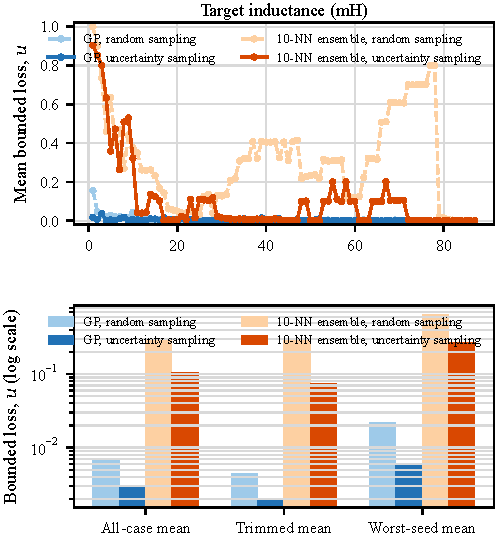
\includegraphics[width=0.90\columnwidth]{fig01_global_surrogate_2x2.pdf}
 \caption{Matched global-surrogate comparison at nominal per-target $B=27$. The upper panel gives all-seed targetwise mean loss; the lower panel gives all-case, targetwise-trimmed, and worst-seed summaries. Every variant models $L$ and $R$ using 17 shared model-building evaluations and the same ten-point target-specific final-evaluation rule.}
 \label{fig:surrogates}
\end{figure}

The ten-network ensemble shows the same directional benefit but remains much less data-efficient. Random sampling qualifies 71.38\% of cases, reaches 274 exact optima, and gives losses of 0.310, 0.285, and 0.649; uncertainty sampling raises qualification to 90.57\%, reaches 651 exact optima, and reduces the losses to 0.104, 0.0745, and 0.268. Active selection therefore helps both model families, while the large remaining gap isolates a model-family and uncertainty-calibration effect rather than a budget or decision-rule advantage.

\subsection{Direct Optimizers}
Fig.~\ref{fig:direct} compares direct-search quality and cost. The trimmed mean loss is 0.0451 for SA, 0.0207 for GA, and 0.0245 for PSO. GA therefore has the lowest mean loss, whereas PSO has the highest untrimmed exact-optimum rate (66.3\% versus 63.9\%) and fewer untrimmed mean evaluations (192.6 versus 203.7; trimmed means 186.5 versus 198.9). PSO is consequently the strongest direct quality--cost/perfection trade-off, not the winner under every statistic. SA requires 92.1 trimmed evaluations (95.1 untrimmed) but is less accurate.

\begin{figure}[!t]
 \centering
 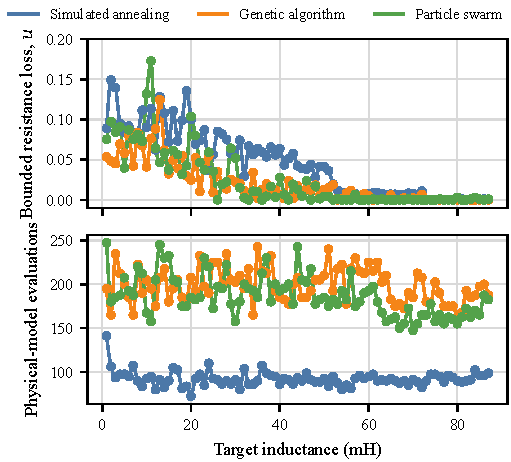
\includegraphics[width=0.90\columnwidth]{fig02_direct_optimizers.pdf}
 \caption{Direct-optimizer comparison. The upper panel gives trimmed bounded loss; the lower panel gives trimmed physical-model evaluations. Each marker is computed at an integer target; shape-preserving splines are included only to aid reading.}
 \label{fig:direct}
\end{figure}

\subsection{Reusable GP Versus Direct Search}
Fig.~\ref{fig:gp-sa} compares global GP uncertainty sampling at $B=27$ with adaptive SA. The GP uses 17 reusable model-building evaluations (six initial and 11 active acquisitions) plus ten final evaluations. Across all ten seeds and 87 targets it qualifies every case; its all-case, trimmed, and worst-seed mean losses are 0.00287, 0.00205, and 0.00611. The head-to-head trimmed mean is therefore 0.00205 for GP and 0.0451 for SA, at 27 nominal evaluations versus 92.1. GP also remains below GA and PSO's trimmed losses while its model-building set is reusable across all targets. Thus all three direct methods are dominated on this benchmark, although this is not evidence of universal GP superiority.

\begin{figure}[!t]
 \centering
 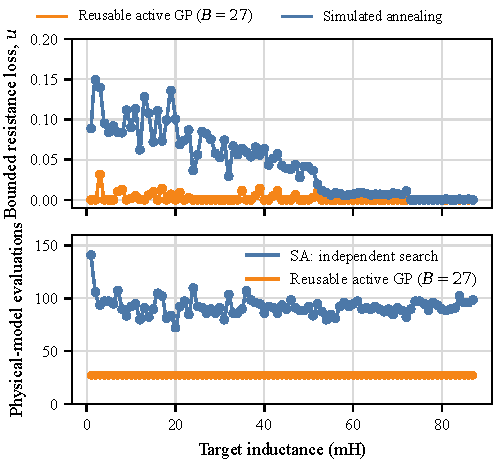
\includegraphics[width=0.90\columnwidth]{fig03_gaussian_process_vs_sa.pdf}
 \caption{Global dual-response GP uncertainty sampling versus simulated annealing. The upper panel gives trimmed bounded loss; the lower panel gives evaluation count. Markers denote every integer target, including all 87 GP observations at $B=27$; splines and connecting lines only aid reading. GP uses 17 shared model-building evaluations and ten target-specific final evaluations. Both use the same $\pm2.5\%$ inductance criterion.}
 \label{fig:gp-sa}
\end{figure}

\section{Target-Conditioned Acquisition}\label{sec:bo-results}
At $B=27$, the selected global GP is the balanced dual-response uncertainty-sampling variant from Fig.~\ref{fig:surrogates}. It qualifies all 870 cases and reaches 740 exact optima, with all-case, targetwise-trimmed, and worst-seed losses of 0.00287, 0.00205, and 0.00611.

All three pure target-conditioned policies qualify every case. Conventional cEI reaches the exhaustive optimum in 867 of 870 cases (99.66\%), with all-case, targetwise-trimmed, and worst-seed mean losses of 0.000161, 0.0000645, and 0.00110. Weighted IVR reaches 827 exact optima and corresponding losses of 0.000819, 0.000554, and 0.00151. Probability-weighted cLCB reaches 829 exact optima and records 0.00274, 0.00108, and 0.00846. Thus cLCB exceeds IVR by two exact recoveries, but IVR has substantially lower loss under every severity summary; their ordering is metric-dependent. cEI remains best by exact recovery and all three loss summaries. At equal standalone-target $B=27$, all three target-conditioned policies improve on the reusable global GP's mean loss.

A fresh 870-case reproducibility audit of the implementation shown in (6), including $\kappa=2$, reproduces every archived decision and loss exactly: 829 optima and mean loss 0.00273805. Thus Fig.~\ref{fig:bo} was generated by the conventional uncertainty-rewarding LCB.

An independent diagnostic over grid locations excluded from each reusable GP fit gives inductance MAE $0.119$~mH and nominal $1\sigma/2\sigma$ empirical coverage of 73.0\%/92.8\%. Absolute error and posterior standard deviation have mean per-seed Pearson correlation 0.534. The uncertainty is therefore informative but imperfectly calibrated: it supports acquisition and stopping, but does not turn the posterior threshold into a coverage or optimality guarantee.

\begin{figure}[!t]
 \centering
 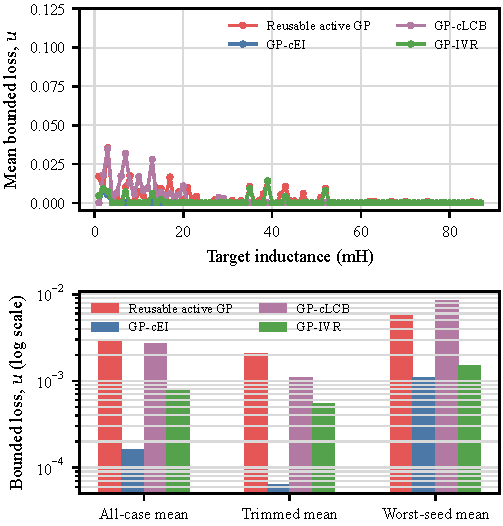
\includegraphics[width=0.90\columnwidth]{fig04_gp_acquisition_comparison.pdf}
 \caption{Matched nominal per-target $B=27$ comparison of the reusable global GP with pure target-conditioned GP-cEI, GP-cLCB, and GP-IVR. The upper panel gives targetwise mean loss; the lower panel gives aggregate summaries. Every method models both $L$ and $R$ and uses the same ten seeds.}
 \label{fig:bo}
\end{figure}

The accounting differs when the entire target library is requested. Independently rerunning a target-conditioned acquisition uses $87\times27=2349$ evaluations, whereas a reusable global model uses $17+87\times10=887$. Target conditioning improves one-query accuracy but costs 2.65 times more for all 87 queries. This precision--generality trade-off makes the allocation of each target-specific budget especially important.

\subsection{Replacing Random Initialization}
The uniform random-six cEI baseline qualifies all 870 cases but misses three exhaustive optima, all at $L_t=2$--3~mH. The deterministic workflow therefore focuses on reliable feasibility discovery rather than further changing the established cEI rule.

Equation~\eqref{eq:feasibility-start} is screened with the same $1+16+10=27$ allocation. Both $\omega=0.75$ and $0.50$ qualify and recover the exact optimum in all 100 target--seed cases. The more conservative $\omega=0.75$ reaches feasibility after a median of six total evaluations, versus eight for $\omega=0.50$. At $\omega=0.25$, all cases qualify but 99 are exact; 60 find feasibility during model building, with a median of 13 evaluations among those 60. The evidence therefore supports a modest 25\% uncertainty share rather than uncertainty-dominated search.

The post-hoc low-target diagnostic provides a complementary stress test. At $L_t=2,3,4,5$~mH, the frozen $\omega=0.75$ rule reaches 40/40 exact optima, whereas random-six cEI reaches 37/40; paired outcomes are three wins, 37 ties, and no losses. Mean bounded loss is zero versus 0.00351. Because these targets were selected after inspecting the baseline failures, this result diagnoses the removed initialization sensitivity but cannot establish general superiority.

An additional pre-optimization screen of 1,000 prespecified random-six designs quantifies how rarely such starts directly cover narrow feasible bands; complete seed-level records are supplied electronically. This screen measures initial coverage only and is not interpreted as downstream GP--cEI failure.

\subsection{Automatic Stopping and GP Reproducibility}
On the combined 14-target screen, the 0.1\% stopping threshold with stochastic GP restarts reaches the exact exhaustive optimum in all 140 cases using 23.743 mean total evaluations. Raising the engineering threshold to 1\% retains 140/140 exact recovery while reducing the mean to 22.593, the median to 23, and the maximum to 26. All trajectories stop naturally before the 27-call cap. The stopping criterion therefore adapts the active budget without removing the terminal evidence batch.

Replacing random GP restarts by the fixed $K=5$ set again yields 140/140 exact records, 22.571 mean calls, median 23, and maximum 26. For each target, all ten nominal seed replays produce identical model-building trajectories, confirmation sets, decisions, and evaluation counts. The seed replays demonstrate software-level invariance; because they collapse to 14 unique trajectories, they are not presented as 140 independent statistical confirmations.

We then give random-six initialization the same 75/25 discovery score, fixed $K=5$ fitting, 1\% stopping rule, ten confirmations, and 27-call ceiling over all 87 targets and ten seeds. It recovers 856/870 exact optima and has seed-dependent decisions at eight targets, versus 87/87 exact deterministic trajectories. Pairing each random case with its target's deterministic result gives 14 deterministic wins, 856 ties, and no losses; mean costs are 22.57 and 21.93 calls, respectively. Because one center and six random observations allocate the active budget differently, this is an operational policy comparison rather than a one-factor proof about initialization alone.

The frozen configuration is then tested once at each of the 73 targets excluded from development. All 73 qualify and recover the exhaustive optimum; all stop naturally. Mean total cost is 21.808 calls, median 22, and range 19--25. Their model-building counts are 9--15, so the $2d+1=5$ guard is inactive and leaves every previously reported 2-D trajectory unchanged. This held-out result removes target-selection overlap and supports generalization across the complete 87-target lattice, while remaining specific to the analytical two-variable oracle.

Calibration is also recomputed from each target-conditioned GP exactly at stopping, before confirmations. Across all unseen grid points, $1\sigma/2\sigma$ coverage is only 44.6\%/77.3\% for $L$ and 56.6\%/86.8\% for $R$, confirming poor global calibration after target-focused sampling. Within each target's true feasible region, coverage improves to 80.8\%/96.5\% for $L$ and 82.1\%/96.3\% for $R$; moreover, the pre-confirmation incumbent is already the exhaustive optimum in all 73 cases. Thus the stopping evidence is locally strong on this oracle, but its posterior remains unsuitable as a global certificate.

Thus the held-out test does not show that ten confirmations are necessary: none improves its incumbent. On the 14-target development set, prefixes of 0, 1, 2, 5, or 10 ranked confirmations likewise retain 140/140 exact replay outcomes. The frozen count is retained as a conservative same-oracle ranking check, not an empirically optimal allocation; it consumes 45.8\% of the held-out mean budget. These calls are neither independent replicates nor higher-fidelity validation.

\begin{figure*}[!t]
 \centering
 \includegraphics[width=0.90\textwidth]{fig05_automated_stopping.pdf}
 \caption{Reproducible automatic budgeting. (a) Mean total calls on the 14-target 2-D development screen; every configuration reaches 100\% exact recovery. (b) Model-building trace for the 8-D WPT transfer. (c) Maximum relative cEI at each feasible-stage refit. Its terminal values are 0.884\%, 0.978\%, and 0.836\%, satisfying the 1\% condition three times; stopping after call 34 is followed by ten confirmations.}
 \label{fig:automatic}
\end{figure*}

\section{Eight-Dimensional WPT Design}
The main WPT screen uses the partial-inductance model as a controlled black-box benchmark rather than an expensive forward solver. Its mixed-integer continuous domain and narrow mutual-inductance band remain nontrivial, while the algorithms receive only queried responses rather than the explicit equations. Although resistance is analytically available to the experimenter, it is deliberately hidden behind the same oracle interface as mutual inductance; fitting two GPs tests the intended setting in which both objective and constraint must be learned under one observation budget. Equal call budgets enable reproducible acquisition and stopping comparisons. These 21-target results measure observation efficiency across numerical electromagnetic models; the separate Maxwell experiment below is an execution demonstration rather than a wall-clock comparison.

The source paper's 15,000 samples (12,000 for training) support a reusable 14-input, multi-pose predictor rather than target-specific optimization. The automated route instead permits $40+10=50$ calls. This is a reuse--specialization cost framing, not a like-for-like algorithm comparison: the active route trades away pose coverage, and optimization accuracy is not prediction accuracy.

An earlier randomly initialized cEI control at $B=50$ qualifies 10/10 seeds with $R=0.3281\pm0.0186~\Omega$ and 1.40\% mean target error. Its nested $B=30,\ldots,80$ sweep qualifies 8/10 seeds at 30 and all seeds thereafter, establishing feasibility but retaining random initialization and fixed budgets.

The frozen transfer screen contains every 50-nH target from 1000 to 2000~nH. With $N_{\min}=2d+1=17$, the automatic and matched-budget conventional policies both qualify 21/21 targets, the center--$p_F$ control qualifies 21/21, and Sobol search qualifies 10/21. Automatic and conventional mean resistances are $0.31500$ and $0.31549~\Omega$; the 0.16\% aggregate difference is not robust dominance (paired wins/ties/losses are 8/3/10, and removing 1250~nH reverses the ordering). The defensible transfer result is reliable feasibility and automatic budgeting, not superior resistance. Table~\ref{tab:wpt-multitarget} retains the original five targets as representative rows; all 21 are supplied electronically.

\begin{table}[!t]
\caption{Matched-budget WPT results and stopping cost. Five representative targets are followed by the complete 21-target aggregate; automatic versus conventional wins/ties/losses are 8/3/10. $R_s$ is the automatic result and $R_{50}$ its forced-$B=50$ continuation.}
\label{tab:wpt-multitarget}
\centering
\scriptsize
\begin{tabular}{@{}rrrrrrr@{}}
\toprule
$M_t$ & $B_s$ & $R_s$ & $R_{50}$ & $\Delta_R$ & Conv. $R_s$ & Sobol $R_s$ \\
\midrule
1000 & 33 & .2597 & .2597 & 0.00\% & .2597 & -- \\
1250 & 34 & .2915 & .2803 & 4.01\% & .3404 & -- \\
1500 & 44 & .3058 & .3058 & 0.00\% & .3056 & .3439 \\
1750 & 27 & .3325 & .3249 & 2.34\% & .3325 & -- \\
2000 & 27 & .3770 & .3437 & 9.69\% & .3711 & .4228 \\
\midrule
Mean (21) & 34.86 & .31500 & .30350 & 3.79\% & .31549 & -- \\
Qualified (21) & -- & 21/21 & 21/21 & -- & 21/21 & 10/21 \\
\bottomrule
\end{tabular}
\end{table}

For the 1500-nH case, the automated configuration first reaches feasibility at model-building call 12 and stops naturally after call 34. Ten simultaneous confirmations give $B=44$. The selected geometry is $(9,7,1.741,61.724,7,7,2.709,61.007)$, ordered as transmitter then receiver $(n_s,n_t,s,r_i)$. Its oracle responses are $M=1466.48$~nH and $R=0.30577~\Omega$. The feasible interval is $[1462.5,1537.5]$~nH, so the design lies only $3.98$~nH (0.265\% of the target) above its lower boundary. This is nominal numerical feasibility with little margin, not evidence of manufacturing or model-discrepancy robustness.

\begin{figure}[!t]
 \centering
 \includegraphics[width=0.82\columnwidth]{fig06_wpt_selected_geometry.pdf}
 \caption{Selected nominal-pose 8-D WPT geometry. The transmitter uses $(n_s,n_t,s,r_i)=(9,7,1.741,61.724)$ and the receiver uses $(7,7,2.709,61.007)$, with lengths in millimetres. Their centers are aligned and their planes are separated by 70~mm; the drawing therefore represents geometry optimization, not a misalignment-tolerance study.}
 \label{fig:wpt-geometry}
\end{figure}

For 1500~nH, the forced control continues from 34 to 40 model-building calls and returns the same design. Across 21 targets, stopping uses 34.86 mean calls, 30.3\% fewer than $B=50$, and returns $0.31500~\Omega$ versus $0.30350~\Omega$, a 3.79\% mean resistance penalty. Twenty runs stop naturally; 1150~nH reaches the declared 40-call safety limit. The benefit is observation efficiency, not runtime or uniformly preserved objective quality.

\subsection{Direct Maxwell Execution}
Table~\ref{tab:maxwell} compares two fully automatic Maxwell trajectories at 1000~nH. The proposed policy starts at the center, discovers feasibility at call 12, and stops after model-building call 20 when relative cEI is 0.887\%, 0.832\%, and 0.878\% on three consecutive refits. Its frozen confirmations improve the feasible incumbent from $0.39671$ to $0.38368~\Omega$. The baseline uses six fixed Sobol points and 14 conventional-cEI calls before the same number of confirmations. Every stored selection replays its declared acquisition exactly, and all 30 geometries in each run are distinct.

\begin{table}[!h]
\caption{Matched 1000-nH Maxwell execution. $J=R_{\rm AC,Tx}+R_{\rm AC,Rx}$ at 85~kHz.}
\label{tab:maxwell}
\centering
\scriptsize
\begin{tabular}{@{}lrr@{}}
\toprule
Metric & Automatic & Sobol-6+cEI-14 \\
\midrule
Model / confirmation calls & $20^\ast/10$ & $20/10$ \\
First feasible call & 12 & 6 \\
Feasible observations & 7/30 & 3/30 \\
Selected $M$ (nH) & 998.929 & 1016.402 \\
Absolute target error & 0.107\% & 1.640\% \\
Selected $J$ ($\Omega$) & \textbf{0.383681} & 0.389535 \\
\bottomrule
\multicolumn{3}{l}{\footnotesize $^\ast$Natural stop; both totals are 30 accepted solver evaluations.}
\end{tabular}
\end{table}

Thus the automatic result is 1.50\% lower in $J$ and produces more feasible evidence under an exactly matched accepted-call budget. Because the baseline already replaces random initialization by a deterministic Sobol design, this pair shows an advantage beyond that substitution alone. It remains one deterministic target per policy: the baseline reaches feasibility earlier, and the result does not establish general field-solver dominance. Moreover, the winning automatic case used the declared 1-mm copper-mesh fallback whereas the baseline winner completed under default adaptive meshing; a common mesh-convergence check is required before interpreting the 1.50\% gap as a definitive high-fidelity objective advantage. The supported claim is direct execution, qualification, and reproducible budget accounting.

\subsection{Dual Application: Resistance-Constrained Coupling}
Some applications specify a winding-resistance ceiling rather than a mutual-inductance target. We therefore reverse the roles and solve
\begin{equation}
 \max_{x\in\mathcal X}M(x)\quad\mathrm{s.t.}\quad R(x)\leq0.35~\Omega .
\end{equation}
The target-aware term becomes constrained expected improvement in $M$, $P(R\leq0.35)\mathrm{EI}_M$; geometry, nominal pose, candidate seeding, and $B=6+32+12=50$ remain unchanged. Pure cEI satisfies the resistance cap in all ten seeds and returns mean best coupling $1824.9\pm165.3$~nH at mean resistance $0.3406~\Omega$. This reversed formulation shows that the same constrained-optimization structure applies when the compulsory target is a ceiling and the optimized response is coupling.

\subsection{Practical Cost and Deployment Choice}
Reusable models amortize construction over many targets; target-conditioned runs specialize calls to one feasible region. Thus the nominal 15,010-versus-44 numerical-WPT arithmetic contrasts multi-pose prediction with one nominal-pose decision, not competing algorithms. A deployable report should separate initialization, adaptive calls, confirmation, failed solver attempts, and accepted observations. Here, $\omega=0.75$, $\delta=1\%$, patience three, $N_{\min}=2d+1$, $K=5$, and ten confirmations are frozen before the reported comparisons. Deployment-task tuning must be charged to its budget; forced $B=50$ is an analysis control, not part of the stopped numerical run.

\subsection{Frozen Deployment Protocol}
After the center evaluation, separate response and objective GPs are refitted. Equation~\eqref{eq:feasibility-start} selects calls until feasibility; cEI and (\ref{eq:stopping}) then govern selection and stopping. Three threshold hits trigger ten simultaneously ranked confirmations, and the final decision is the best feasible oracle observation, never a prediction. On transfer, only candidate realization changes: the lattice becomes 2048-point deterministic Sobol blocks per refit and a 4096-point confirmation block. Candidate counts are disclosed although they are not physical calls. Noisy deployment would additionally require charged replicates or a declared noise model.

\subsection{Reproducibility Package}
The public repository at \url{https://github.com/le-dong-xjtu/reproducible-target-informed-gp} retains raw data, manifests, experiment and rendering scripts, and an evidence map from claims to inputs and code. Its validation scripts recompute losses, budgets, histories, stopping summaries, replay identity, numerical WPT decisions, and the matched Maxwell records; superseded artifacts are marked historical.

\section{Interpretation and Limitations}
The study separates reusable representation, target conditioning, sparse-data feasibility discovery, reproducible GP fitting, and budget allocation. Results favor cEI for single-target precision and support posterior-improvement stopping with a terminal evidence batch. The center removes initialization randomness, $\omega$ exposes the feasibility/exploration preference, and fixed low-discrepancy starts replace a seed by allowance $K$.

The evidence does not establish universal superiority or defaults. Although the frozen test covers all 73 unused lattice targets, $\omega=0.75$ was selected on ten development targets and the 2--5~mH diagnostic is post-hoc. The 1,000-seed screen concerns initial feasible coverage rather than complete acquisition trajectories. The numerical WPT screen covers 21 targets but one nominal pose and deterministic trajectory each; the Maxwell evidence is only one target and one trajectory per policy. Discontinuity, noise, kernel misspecification, or sparse candidates can invalidate calibration and the 1\% threshold. The field-solver pair demonstrates executable transfer but, without a common mesh-convergence check or repeated targets, does not independently validate the numerical oracle or prove optimizer superiority. Experimental hardware, fabrication, thermal behavior, efficiency, misalignment, and model-discrepancy robustness remain outside scope. The 15,000-label comparison is only a reuse--specialization cost framing.

\section{Conclusion}
Active dual-response GP and target-conditioned cEI are the strongest tested choices on the 2-D lattice. The reproducible configuration adds a center start, 75/25 feasibility discovery, fixed $K=5$ GP starts, a $2d+1$ minimum, relative-cEI stopping, and explicit confirmations. It recovers all 73 held-out optima; both GP policies qualify all 21 numerical WPT targets without a robust resistance difference. In the matched 1000-nH Maxwell demonstration, the automatic policy also qualifies with seven feasible observations and $J=0.38368~\Omega$, versus three and $0.38954~\Omega$ for Sobol-initialized cEI. This single direct execution strengthens engineering plausibility while leaving the supported contribution as explicit, reproducible allocation of constrained-design observations rather than universal optimizer superiority.

\balance
\begin{thebibliography}{00}
\fontsize{6.5}{7.1}\selectfont
\bibitem{rasmussen} C. E. Rasmussen and C. K. I. Williams, \emph{Gaussian Processes for Machine Learning}. MIT Press, 2006.
\bibitem{settles} B. Settles, ``Active Learning Literature Survey,'' University of Wisconsin--Madison, Computer Sciences Technical Report 1648, 2009.
\bibitem{lakshminarayanan} B. Lakshminarayanan, A. Pritzel, and C. Blundell, ``Simple and scalable predictive uncertainty estimation using deep ensembles,'' in \emph{Advances in Neural Information Processing Systems}, 2017.
\bibitem{kirkpatrick} S. Kirkpatrick, C. D. Gelatt, Jr., and M. P. Vecchi, ``Optimization by simulated annealing,'' \emph{Science}, vol. 220, no. 4598, pp. 671--680, May 1983, doi: 10.1126/science.220.4598.671.
\bibitem{holland} J. H. Holland, \emph{Adaptation in Natural and Artificial Systems}. University of Michigan Press, 1975.
\bibitem{kennedy} J. Kennedy and R. Eberhart, ``Particle swarm optimization,'' in \emph{Proc. ICNN'95---Int. Conf. Neural Networks}, vol. 4, Perth, WA, Australia, 1995, pp. 1942--1948, doi: 10.1109/ICNN.1995.488968.
\bibitem{gardner} J. Gardner, M. Kusner, Z. Xu, K. Weinberger, and J. Cunningham, ``Bayesian optimization with inequality constraints,'' in \emph{Proc. 31st Int. Conf. Mach. Learn.}, PMLR, vol. 32, pp. 937--945, 2014.
\bibitem{srinivas} N. Srinivas, A. Krause, S. M. Kakade, and M. Seeger, ``Gaussian process optimization in the bandit setting: No regret and experimental design,'' in \emph{Proc. 27th Int. Conf. Mach. Learn.}, 2010, pp. 1015--1022.
\bibitem{cohn} D. A. Cohn, Z. Ghahramani, and M. I. Jordan, ``Active learning with statistical models,'' \emph{J. Artif. Intell. Res.}, vol. 4, pp. 129--145, 1996, doi: 10.1613/jair.295.
\bibitem{asadi2025} M. Asadi and A. M. Abazari, ``A data-driven model to predict mutual inductance between planar coils with arbitrary specifications and positions,'' \emph{IET Electr. Power Appl.}, vol. 19, Art. no. e70015, 2025, doi: 10.1049/elp2.70015.
\bibitem{liu2014} B. Liu, H. Aliakbarian, Z. Ma, G. A. E. Vandenbosch, G. Gielen, and P. Excell, ``An efficient method for antenna design optimization based on evolutionary computation and machine learning techniques,'' \emph{IEEE Trans. Antennas Propag.}, vol. 62, no. 1, pp. 7--18, Jan. 2014, doi: 10.1109/TAP.2013.2283605.
\bibitem{wu2024} Q. Wu, W. Chen, C. Yu, H. Wang, and W. Hong, ``Machine-learning-assisted optimization for antenna geometry design,'' \emph{IEEE Trans. Antennas Propag.}, vol. 72, no. 3, pp. 2083--2095, Mar. 2024, doi: 10.1109/TAP.2023.3346493.
\bibitem{sim2023} B. Sim \emph{et al.}, ``Bayesian optimization based fast and accurate wireless power transfer system coil optimization for high efficiency,'' in \emph{Proc. IEEE Wireless Power Technology Conf. Expo. (WPTCE)}, 2023, doi: 10.1109/WPTCE56855.2023.10215668.
\bibitem{furuuchi2024} S. Furuuchi and S. Yamada, ``Verifying the effect of initial sample size in Bayesian optimization,'' \emph{Total Quality Science}, vol. 10, no. 1, pp. 8--19, 2024, doi: 10.17929/tqs.10.8.
\bibitem{ishibashi2023} H. Ishibashi, M. Karasuyama, I. Takeuchi, and H. Hino, ``A stopping criterion for Bayesian optimization by the gap of expected minimum simple regrets,'' in \emph{Proc. 26th Int. Conf. Artificial Intelligence and Statistics}, PMLR, vol. 206, pp. 6463--6497, 2023.
\bibitem{zhang2019mept} W. Zhang, X. Wu, C. Xia, and X. Liu, ``Maximum efficiency point tracking control method for series--series compensated wireless power transfer system,'' \emph{IET Power Electron.}, vol. 12, no. 10, pp. 2534--2542, Aug. 2019, doi: 10.1049/iet-pel.2018.5610.
\bibitem{ansysloss} Ansys, ``Per-winding loss outputs for Maxwell 2D/3D transient and eddy current designs,'' \emph{Ansys Electronics Desktop Help}, 2024 R2. [Online]. Available: https://ansyshelp.ansys.com/
\end{thebibliography}

\end{document}
